\section{Multithreading}
\hspace*{0.5in} Menjalankan beberapa\textit{ thread} mirip dengan menjalankan beberapa program yang berbeda secara bersamaan, namun dengan manfaat berikut : \par

\begin{itemize}
\item Beberapa \textit{thread} dalam proses berbagi ruang data yang sama dengan benang induk dan karena dapat saling berbagi informasi atau berkomunikasi satu sama lain dengan lebih muda daripada jika prosesnya terpisah \par

\item \textit{thread} terkadang disebut proses ringan dan tidak membutuhkan banyak memori atas, mereka lebih murah daripada proses.\end{itemize}
\par

\vspace{12pt}
\hspace*{0.5in} Sebuah \textit{thread} memiliki permulaan, urutan eksekusi dan sebuah kesimpulan. Ini memiliki pointer perintah yang melacak dari mana dalam konteksnya saat ini berjalan. \par

\begin{itemize}
\item Hal ini dapat dilakukan sebelum pre-\textit{empted} (\textit{inturrepted})\end{itemize}
\par
\noindent 
\begin{itemize}
\item Untuk sementara dapat ditunda sementara \textit{thread} lainnya yang sedang berjalan ini disebut unggul. \end{itemize}
\par
\noindent 
\subsection{Memulai Thread Baru} \par
\noindent 
\hspace*{0.5in} Untuk melakukan \textit{thread} lain, perlu memanggil metode berikut yang tersedia dimodul \textit{thread} : \par
\noindent 
\begin{center}{\fontsize{9pt}{9pt}\selectfont Thread.start $  \_  $new $  \_  $thread (function, args [, kwargs] )}\end{center} \par
Pemanggilan metode ini memungkinkan cara cepat dan tepat untuk membuat \textit{thread} baru di linux dan window. \par
\hspace*{0.5in} Pemanggilan metode segera kembali dan anak  \textit{thread} dimulai dan fungsi pemanggilan dengan daftar \textit{args} telah berlalu. Saat fungsi kembali ujung \textit{thread} akan berakhir. Disini, \textit{args }adalah tupel argumen. Gunakan tupel kosong untuk memanggil fungsi tanpa melewati argumen. \textit{Kwargs} adalah kamus opsional argumen kata kunci.  \par

\vspace{12pt}
Contoh : 
\begin{verbatim}
\#  $!/usr/bin/python} 

Import thread
Import time

#  $ Define a function for the thread 

Def print $  \_  $time (threadNamw, delay):
Count = 0
While count <5:
Time.sleep(delay)
Count +=1 
Print  $ " $ $  \%  $s :  $  \%  $s $ " $  $  \%  $ 
(threadName, time.ctime(time.time()))

#  $ Create two thread as follows
try:
thread.start $  \_  $new $  \_  $thread(print $  \_  
$time, ( $ " $Thread-1 $ " $, 2, ))
thread.start $  \_  $new $  \_  $thread(print $  \_  
$time, ( $ " $Thread-2 $ " $, 4,))
except: 
print " $Error: unable to start thread 

while 1:
pass 
\end{verbatim}

\vspace{80pt}	
Bila kode diatas dieksekusi, maka menghasilkan hasil sebagai berikut : \par
\vspace{10pt}
\noindent 
\begin{center}{\fontsize{10pt}{10pt}\selectfont Thread-1 : Thu Jan 22 15:42:17 2009}\end{center} \par
\noindent 
\begin{center}{\fontsize{10pt}{10pt}\selectfont Thread-1 : Thu Jan 22 15:42:19 2009}\end{center} \par
\noindent 
\begin{center}{\fontsize{10pt}{10pt}\selectfont Thread-2 : Thu Jan 22 15:42:19 2009}\end{center} \par
\noindent 
\begin{center}{\fontsize{10pt}{10pt}\selectfont Thread-1 : Thu Jan 22 15:42:21 2009}\end{center} \par
\noindent 
\begin{center}{\fontsize{10pt}{10pt}\selectfont Thread-2 : Thu Jan 22 15:42:23 2009}\end{center} \par
\noindent 
\begin{center}{\fontsize{10pt}{10pt}\selectfont Thread-1 : Thu Jan 22 15:42:23 2009}\end{center} \par
\noindent 
\begin{center}{\fontsize{10pt}{10pt}\selectfont Thread-1~:  Thu Jan 22 15:42:23 2009}\end{center} \par
\noindent 
\begin{center}{\fontsize{10pt}{10pt}\selectfont Thread-1 : Thu Jan 22 15:42:25 2009}\end{center} \par
\noindent 
\begin{center}{\fontsize{10pt}{10pt}\selectfont Thread-2 : Thu Jan 22 15:42:27 2009}\end{center} \par
\noindent 
\begin{center}{\fontsize{10pt}{10pt}\selectfont Thread-2 : Thu Jan 22 15:42:31 2009}\end{center} \par
\noindent 
\begin{center}{\fontsize{10pt}{10pt}\selectfont Thread-2 : Thu Jan 22 15:42:35 2009}\end{center} \par

\vspace{12pt}
\hspace*{0.5in} Meskipun sangat efektif untuk benang tingkat rendah, namun modul \textit{thread} sangat terbatas dibandingkan dengan modul yang baru. \par

\vspace{12pt}
\subsection {Modul Threading} \par
\hspace*{0.5in} Modul threading yang lebih baru disertakan dengan Python 2.4 memberikan jauh lebih kuat, dukungan tingkat tinggi untuk \textit{thread}\textit{ }dari modul\textit{ }\textit{thread}\textit{ }dibahas pada bagian sebelumnya. \par
\hspace*{0.5in} The \textit{thread}\textit{ing }modul mengekpos semua metode dari \textit{thread}\textit{ }dan menyediakan beberapa metode tambahan : \par

\begin{itemize}
\item \textbf{t}\textbf{hreading.activeCount() } \par
Mengembalikan jumlah objek \textit{thread} yang aktif \par
\item \textbf{t}\textbf{hreading.currentThread() } \par
Mengembalikan jumlah objek \textit{thread} dalam kontrol benang pemanggil \par
\item \textbf{t}\textbf{hreading.enumerate() } \par
Mengembalikan daftar semua benda \textit{thread}\textit{ }yang sedang aktif \par

\vspace{12pt}
\hspace*{0.5in} Selain metode, modul \textit{thread}\textit{ing }memiliki \textit{thread}\textit{ }kelas yang mengimplementasikan \textit{thread}\textit{ing. }Metode yang disediakan oleh \textit{thread}\textit{ }kelas adalah sebagai berikut : \par
\item \textbf{run()} \par
Metode adalah titik masuk untuk \textit{thread} \par
\item \textbf{start()} \par
Metode dimulai\textbf{ }\textit{thread}\textit{ }dengan memanggil metode run \par
\item \textbf{join(}\textbf{[time]}\textbf{)} \par
Menunggu benang untuk mengakhiri \par
\item \textbf{isAlive()} \par
Metode memeriksa apakah\textbf{ }\textit{thread}\textit{ }masih mengeksekusi\textbf{ } \par
\item \textbf{getName()} \par
Metode mengambalikan nama\textbf{ }\textit{thread} \par
\item \textbf{setName()} \par
Metode menetapkan nama\textbf{ }\textit{thread} \par

\vspace{12pt}
\subsection {Membuat Thread Menggunakan Modul} \par
\hspace*{0.5in} Untuk melaksanakan \textit{thread}\textit{ }baru menggunakan\textit{ threading} harus melakukan hal berikut : \par
\item Mendefinisikan subclass dari \textit{thread} kelas \par
\item Menimpa  $  \_  $init $  \_  $ (self [args]) metode untuk menambahkan argumen tambahan \par
\item Menimpa run(self[args]) metode untuk menerapkan apa \textit{thread} harus dilakukan ketika mulai 
\end{itemize}

\vspace{12pt}
\hspace*{0.5in} Setelah membuat baru \textit{thread} subclass, dapat membuah seuah instance dari itu dan kemudian memulai \textit{thread} baru dengan menerapkan \textit{start(),} yang ada gilirinnya panggilan \textit{run()} metode. \par
\vspace{50pt}

Contoh :
\begin{verbatim} 
#  $!/usr/bin/python

import threading
import time

exitFlag = 0

class myThread (threading.Thread): 
def $  \_  $init $  \_  $(self, threadID, name, 
counter) :
threading.Thread. $  \_  $init $  \_  $(self)} 
self.threadID = threadID
self.name = name 
self.counter = counter 
def run (self) :
print  $ " $Starting  $ " $ + self.name 
print $  \_  $time(self.name, self.counter, 5)
print  $ " $Exiting  $ " $+ self.name

def print $  \_  $time(threadName, delay, counter):} 

while counter:

if exitFlag: 
threadName.exit() 
time.sleep(delay) 
print  $ " $ $  \%  $s:  $  \%  $s $ " $  $  \%  
$ (threadName, time.ctime(time.time()))
counter -= 1} 

#  $ Create new threads
thread1 = myThread(1,  $ " $Thread-1 $ " $, 1)
thread2 = myThread(2,  $ " $Thread-2 $ " $, 2)
#  $ Start new threads
thread1.start()
thread2.start()
print  $ " $Exiting Main Thread $ " $
\end{verbatim}

\vspace{12pt}
Ketika kode diatas dijalankan, menghasilkan hasil sebagai berikut:
\par
\noindent 
{\fontsize{10pt}{10pt}\selectfont Starting Thread-1} \par
\noindent 
{\fontsize{10pt}{10pt}\selectfont Starting Thread-2} \par
\noindent 
{\fontsize{10pt}{10pt}\selectfont Exiting Main Thread} \par
\noindent 
{\fontsize{10pt}{10pt}\selectfont Thread-1 : Thu Mar 21 09:10:03 2013} \par
\noindent 
{\fontsize{10pt}{10pt}\selectfont Thread-1 : Thu Mar 21 09:10:04 2013} \par
\noindent 
{\fontsize{10pt}{10pt}\selectfont Thread-2 : Thu Mar 21 09:10:04 2013} \par
\noindent 
{\fontsize{10pt}{10pt}\selectfont Thread-1 : Thu Mar 21 09:10:05 2013} \par
\noindent 
{\fontsize{10pt}{10pt}\selectfont Thread-2 : Thu Mar 21 09:10:06 2013} \par
\noindent 
{\fontsize{10pt}{10pt}\selectfont Thread-1 : Thu Mar 21 09:10:07 2013} \par
\noindent 
{\fontsize{10pt}{10pt}\selectfont Exiting Thread-1} \par
\noindent 
{\fontsize{10pt}{10pt}\selectfont Thread-2 : Thu Mar 21 09:10:08 2013} \par
\noindent 
{\fontsize{10pt}{10pt}\selectfont Thread-2 : Thu Mar 21 09:10:10 2013} \par
\noindent 
{\fontsize{10pt}{10pt}\selectfont Thread-2 : Thu Mar 21 09:10:12 2013} \par
\noindent 
{\fontsize{10pt}{10pt}\selectfont Exiting Thread=2} \par

\vspace{10pt}
\subsection{Sinkronisasi Thread} \par
\hspace*{0.5in} \textit{T}\textit{hread}\textit{ing }modul disediakan dengan Python termasuk sederhana untuk menerapkan mekanisme bahwa memungkinkan untuk menyinkronkan \textit{thread}\textit{ }penguncian. Sebuah kunci baru dibuat dengan memanggil \textit{lock() }metode yang mengembalikan kunci baru. \par
\hspace*{0.5in} The \textit{acquire}\textit{ }\textit{(blocking)}\textit{ }metode objek kunci baru digunakan untuk memaksa \textit{thread}\textit{ }untuk menjalankan serempak. Opsional \textit{blocking} parameter memungkikan untuk mengontrol apakah\textit{ thread} menunggu untuk mendapatkan kunci. \par
\hspace*{0.5in} Jika \textit{blocking} diatur ke 0, \textit{thread} segera kembali dengan nilai 0 jika kunci tidak dapat diperoleh dan dengan 1 jika kunci dikuisisi. Jika pemblokiran diatur ke 1, blok dan menunggu kunci yang akan dirilis. \par
\hspace*{0.5in}The \textit{release()} metode objek kunci baru digunakan untuk melepaskan kunci ketika tidak lagi diperlukan.  \par
\noindent 

\vspace{12pt}
Contoh: 
\begin{verbatim}
#  $!/usr/bin/python

import threading
import time

class myThread (threading.Thread): 
def $  \_  $init $  \_  $(self, threadID, name, 
counter):
threading.Thread. $  \_  $init $  \_  $(self)
self.threadID = threadID
self.name = name
self.counter = counter
def run(self) 
print  $ " $Starting  $ " $+ self.name 
$  \#  $ Get lock to synchronize threads 
ThreadLock.acquire() 
print $  \_  $time(self.name, self.counter, 3) 
#  $ Free lock to realease next thread
ThreadLock.release()
Def print $  \_  $time(threadName, delay, counter):
while counter:
time.sleep(delay)
print  $ " $ $  \%  $s:  $  \%  $s $ " $  $  \%  $ 
(threadName, time.ctime(time.time()))
counter -= 1
threadLock = threading.Lock() 
threads = []
#  $ Create new threads
thread1 = myThread(1,  $ " $Thread-1,1 ) 
thread2 = myThread(2,  $ " $Thread-2,2 )
#  $ Start new Threads} 
thread1.start() 
thread2.start()

#Add threads to thread list} 
threads.append(thread1)} 
thread2.append(thread2)} 
\vspace{10pt}

#  $ Wait for all threads to complete}  
Fort t in threads:
t.join()
print  $ " $Exiting Main thread $ " $
\end{verbatim}

\vspace{8pt}
Bila kode diatas dieksekusi, maka menghasilkan sebagai berikut : \par
{\fontsize{10pt}{10pt}\selectfont Starting Thread-1} \par
\noindent 
{\fontsize{10pt}{10pt}\selectfont Starting Thread-2} \par
\noindent 
{\fontsize{10pt}{10pt}\selectfont Thread-1: Thu Mar 21 09:11:28 2013} \par
\noindent 
{\fontsize{10pt}{10pt}\selectfont Thread-1: Thu Mar 21 09:11:29 2013} \par
\noindent 
{\fontsize{10pt}{10pt}\selectfont Thread-1: Thu Mar 21 09:11:30 2013} \par
\noindent 
{\fontsize{10pt}{10pt}\selectfont Thread-2: Thu Mar 21 09:11:32 2013} \par
\noindent 
{\fontsize{10pt}{10pt}\selectfont Thread-2: Thu Mar 21 09:11:34 2013} \par
\noindent 
{\fontsize{10pt}{10pt}\selectfont Thread-2: Thu Mar 21 09:11:36 2013} \par
\noindent 
{\fontsize{10pt}{10pt}\selectfont Exiting Main Thread} \par

\vspace{8pt}
\subsection{Multithreaded Antrian Prioritas} \par
\hspace*{0.5in} The queue modul memungkinkan untuk membuat objek antrian baru yang dapat menampung jumlah tertentu item. Ada metode berikut untuk mengontrol antrian : \par
\vspace{15pt}
\begin{itemize}
	\item \textbf{get()} \par
		Menghapus dan mengembalikan item dari antrian
	\par
	\item \textbf{put()} \par
		Menambahkan item ke antrian
	\par
	\item \textbf{qsize()} \par
		Mengembalikan jumlah item yang saat ini dalam antrian
	\par
	\item \textbf{empty()} \par
		Mengembalikan benar jika antrian kosong jika tidak, salah
	\par
	\item \textbf{full()}\end{itemize}
\par
	Mengembalikan benar jika antrian penuh jika tidak, salah

\vspace{12pt}
Contoh:  
\begin{verbatim}
#  $!/usr/bin/python}  

import Queue
import threading
import time

exitFlag = 0 

class myThread (threading.Thread): 
def   $  \_  $init $  \_  $(self, threadID, name, q):
threading.Thread. $  \_  $init $  \_  $(self) 
self.name = name
self.q = q
def run(self):
print  $ " $Starting  $ " $+ self.name
process $  \_  $data(self.name, self.q) 
print  $ " $Exiting  $ " $+ self.name 
def process $  \_  $data(threadName, q):
while not exitFlag:
queuLock.acquire()
if not workQueu.empty(): 
data = q.get() 
queueLock.release() 
print  $ " $ $  \%  $s processing  $  \%  $s $ " $ 
$  \%  $ (threadName, data) 
else: 
queueLock.release()
time.sleep(1) 

threadList = [ $ " $Thread-1 $ " $,  $ " $Thread-2 $
" $,  $ " $Thread-3 $ " $]
nameList = [ $ " $One $ " $,  $ " $Two $ " $,  $ "
$Three $ " $,  $ " $Four $ " $,  $ " $Five $ " $]
queueLock = threading.Lock()
workLock = Queue.Queue(10)
threads = [] 
threadID = 1 

#  $ Create new threads
For tName in threadList: 
thread = myThread(threadID, tName, workQueue)
thread.start()
thread.append(thread)
threadID +=1

#  $ Fill the queue 
queueLock.acquire() 
for word in nameList:
workQueue.put(word) 
queueLock.release()

#  $ Wait for queue to empty
while not workQueue.empty(): 
pass 

#  $ Notify threads it?s time to exit
exitFlag = 1

#  $ Wait for all threads to complete
For t in threads:
t.join()
print  $ " $Exiting Main Thread $ " $
\end{verbatim}

\vspace{10pt} 
Bila kode diatas dieksekusi, maka menghasilkan hasil sebagai berikut: \par
\vspace{12pt}
\noindent 
{\fontsize{10pt}{10pt}\selectfont Starting Thread-1} \par
\noindent 
{\fontsize{10pt}{10pt}\selectfont Starting Thread-2} \par
\noindent 
{\fontsize{10pt}{10pt}\selectfont Starting Thread-3} \par
\noindent 
{\fontsize{10pt}{10pt}\selectfont Thread-1 processing One} \par
\noindent 
{\fontsize{10pt}{10pt}\selectfont Thread-2 processing Two} \par
\noindent 
{\fontsize{10pt}{10pt}\selectfont Thread-3 processing Three} \par
\noindent 
{\fontsize{10pt}{10pt}\selectfont Thread-1 processing Four} \par
\noindent 
{\fontsize{10pt}{10pt}\selectfont Thread-2 processing Five} \par
\noindent 
{\fontsize{10pt}{10pt}\selectfont Exiting Thread-3} \par
\noindent 
{\fontsize{10pt}{10pt}\selectfont Exiting Thread-1} \par
\noindent 
{\fontsize{10pt}{10pt}\selectfont Exiting Thread-2} \par
\noindent 
{\fontsize{10pt}{10pt}\selectfont Exiting Main Thread} \par

\section{Cara menggunakan Threading untuk Membuat Benang}
\hspace*{0.5in} Threading menggabungkan semua metode thread dan menampilkan beberapa metode tambahan. Terlepas dari metode di atas, threading juga menyajikan kelas Thread yang dapat dicoba untuk mengimplementasikan thread. Ini adalah varian object-oriented dari multithreading Python. Kelas <Thread> menerbitkan metode berikut :

\begin{table}[ht]
	\caption{Ukuran}
	\begin{tabular*}{\textwidth}{@{\extracolsep{\fill}}lcc}
		\hline
		Kelas&  Penjelasan Metode&\cr
		\hline
		run():&Ini adalah fungsi entry point untuk thread manapun&\cr
		start():&Metode start () memicu thread saat metode dijalankan dipanggil&\cr
		join([time]):&Metode join () memungkinkan sebuah program untuk menunggu thread untuk diakhiri&\cr
		\hline
	\end{tabular*}
	\begin{tablenotes}
	\end{tablenotes}
\end{table}

\section{Mengimplementasikan Thread menggunakan Threading}
\hspace*{0.5in} Buatlah subkelas dari kelas Thread. Timpa metode (self [, args]) untuk memberi argumen sesuai persyaratan. Selanjutnya, timpa metode run (self [args]) untuk mengkodekan logika bisnis benang.

\hspace*{0.5in} Setelah mendefinisikan subclass Thread baru, harus memberi instantiate untuk memulai thread baru. Berikut \ref{Mengimplementasikan Thread menggunakan Threading} Mengimplementasikan Thread menggunakan Threading :
\begin{figure}[ht]
	\centerline{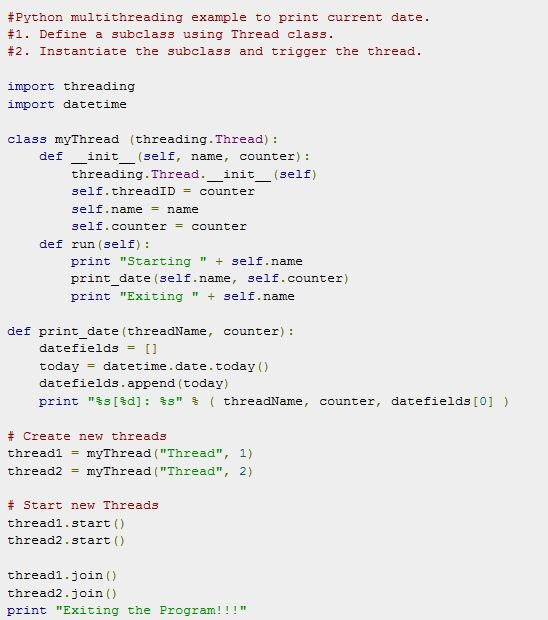
\includegraphics[width=0.75\textwidth]{figures/Thread}}
	\caption{Mengimplementasikan Thread menggunakan Threading}
	\label{Mengimplementasikan Thread menggunakan Threading}
\end{figure}
